% !TEX root = ../report.tex
\section{Das Partikelsystem}
\begin{Spacing}{\mylinespace}

Nachdem wir im ersten Projektsemester mit unserem CPU-basierten Partikelsystem sehr schnell an die Grenzen des machbaren gestoßen waren, haben wir uns im zweiten Projektsemester kurzfristig dafür entschieden, das System noch einmal komplett zu überarbeiten und dieses Mal auf eine reine GPU Implementierung zu setzen.

\subsection{Die Anforderungen}

Als Anforderungen haben wir uns gesetzt, ein hoch flexibles und vom restlichen System getrenntes Partikelsystem zu entwickeln, welches die Fähigkeit bietet mehrere hunderttausend oder sogar Millionen von Partikeln in Echtzeit darzustellen.  

\subsection{Die Umsetzung}

Um unser angestrebtes Ziel zu erreichen, haben wir auf eine Kombination aus verschiedenen Techniken gesetzt, die wir folgend etwas genauer Beschreiben werden.
 
\begin{description}
	\item[Billboarding] \hfill \\
	Für die Darstellung unserer Partikel haben wir zwei unterschiedliche Techniken in Betracht gezogen. Bei der erste und einfacheren Technik wird ein Partikel durch einen einzelnen Vertex repräsentiert und anschließend, als farbiger Punkt, auf den Bildschirm gezeichnet. Da wir aber nicht auf die Möglichkeit verzichten wollten, bei Bedarf unseren Partikeln auch eine Textur zuzuweisen, haben wir uns für die zweite, etwas aufwendigere, Technik das \textit{Billboarding} entschieden.
\\\\
\textit{Billboards} bestehen aus zwei dreieckigen Polygonen die ein Rechteck bilden (s. Abbildung \ref{fig:BBQuad}).	Dieses Rechteck wird anschließend im Vertexshader, mit Hilfe der Viewmatrix der Kamera, so transformiert damit es immer in Richtung des Betrachters ausgerichtet ist. Durch diese Eigenschaft, lassen sich, mit sehr geringem Rechenaufwand, unterschiedlichste Effekte realisieren. In unserem Anwendungsfall, die Darstellung von Rauch beziehungsweise Nebel. 

\begin{figure}[h!]
	\centering
	\vspace*{30px}
	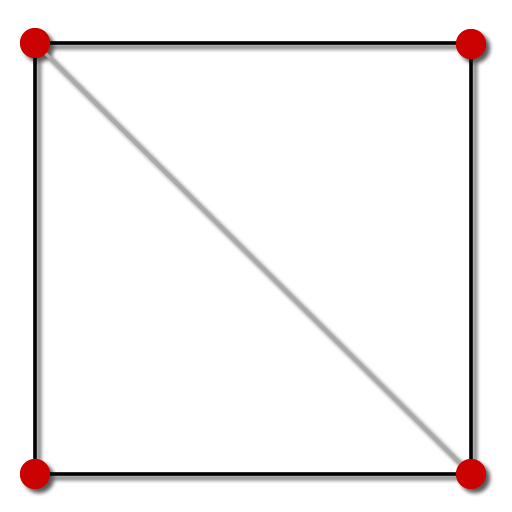
\includegraphics[width=110px]{graphics/billboardQuad.png}
	\caption{Aufbau des Rechtecks für ein Billboard.}
	\label{fig:BBQuad}
\end{figure}
\newpage
	\item[Instancing] \hfill \\
	Bei dieser Technik handelt es sich, um eine von der Grafikhardware bereitgestellten Funktionalität, zur Reduzierung von sogenannten \textit{Drawcalls}. Unter einem \textit{Drawcall} versteht man im Allgemeinen, das Zeichen eines Objekt mit einem bestimmten Material, einer Transformation und gegebenenfalls weiteren Eigenschaften. In unserem Fall wäre also jedes gezeichnete Partikel (Billboard) ein \textit{Drawcall}. Diese sind allerdings sehr teuer und bei der angestrebten Anzahl von über 1.000.000 Partikeln, wäre an eine Echtzeitfähigkeit nicht mehr zu denken gewesen. Somit entschieden wir uns für das \textit{Instancing}. Diese Technik erlaubt es 1.048.576 Instanzen der gleichen Geometrie, in unserem Fall die Billboards, in nur einem einzigen \textit{Drawcall} zu Zeichen. 
	
	\item[Rendertargets] \hfill \\
	In unserer vorherigen CPU-basierten Implementierung des Partikelsystems, war es ein leichtes, die benötigten Eigenschaften (Position, Geschwindigkeit, usw.) unserer Partikel, in einer dazu passenden Datenstruktur im RAM abzulegen und zu manipulieren. Bei der Neuimplementierung musste nun ein Weg gefunden werden, die Speicherung und Manipulation der Partikeleigenschaften, performant auf die GPU zu übertragen.
\\\\
Hierfür entschieden wir uns, für die Nutzung sogenannter \textit{Rendertargets}.   Diese repräsen- tieren eine spezielle Art von Texturen, für die neben dem standardmäßigen Lesezugriff auch Schreibzugriff zur Verfügung steht. Durch diese Eigenschaft, wird es möglich, \textit{Rendertargets} als Datencontainer zu nutzen und deren Inhalt direkt auf der GPU zu manipulieren.
\\\\
Zusätzlich zu den normalen \textit{Rendertargets}, unterstützt XNA auch \textit{Multiple Rendertargets}. Welche es ermöglichen, während eines Passes, in bis zu vier Rendertargets gleichzeitig zu schreiben.
\\\\
Mit dieser Technik war es uns nun möglich, unsere einzelnen Partikeleigenschaften in den einzelnen Farbkanälen der vier verfügbaren Rendertargets abzulegen (s. Abbildung \ref{fig:RTCahnnels}) und direkt auf der GPU zu manipulieren. 
	
\begin{figure}[h!]
	\centering
	\vspace*{55px}
	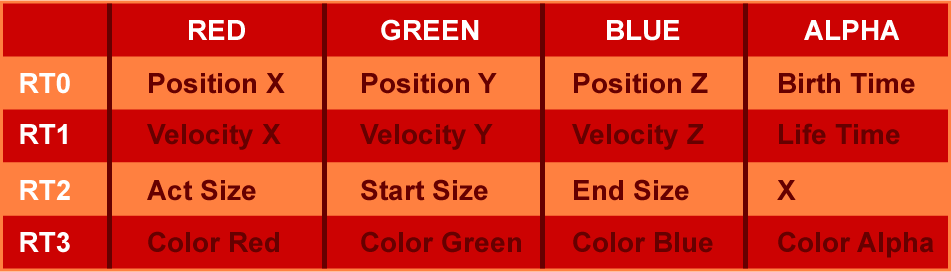
\includegraphics[width=410px]{graphics/RendertargetsChannels.png}
	\caption{Kanalbelegung der einzelnen Rendertargets.}
	\label{fig:RTCahnnels}
\end{figure}	
	
	\item[Ping-Pong] \hfill \\
	Im Normalfall können \textit{Rendertargets}, innerhalb eines Passes, entweder nur gelesen oder nur geschrieben werden. Um diese Einschränkung zu umgehen und einen weiteren Pass einzusparen, setzten wir das sogenannte \textit{Ping-Pong} Verfahren ein. Bei diesem Verfahren, existiert von jedem \textit{Rendertarget} ein Duplikat (s. Abbildung \ref{fig:DoubleTarget}). Während eines Passes wird nun eines der Duplikate genutzt um Daten daraus zu lesen und das andere um die manipulierten Daten zurück zuschreiben. Im Anschluss an den Pass, werden die beiden \textit{Rendertargets} dann einfach ausgetauscht. Somit können im nächsten Pass, die zuvor geschrieben Daten gelesen werden und die alten Daten können überschrieben werden.
	
\begin{figure}[h!]
	\centering
	\vspace*{30px}
	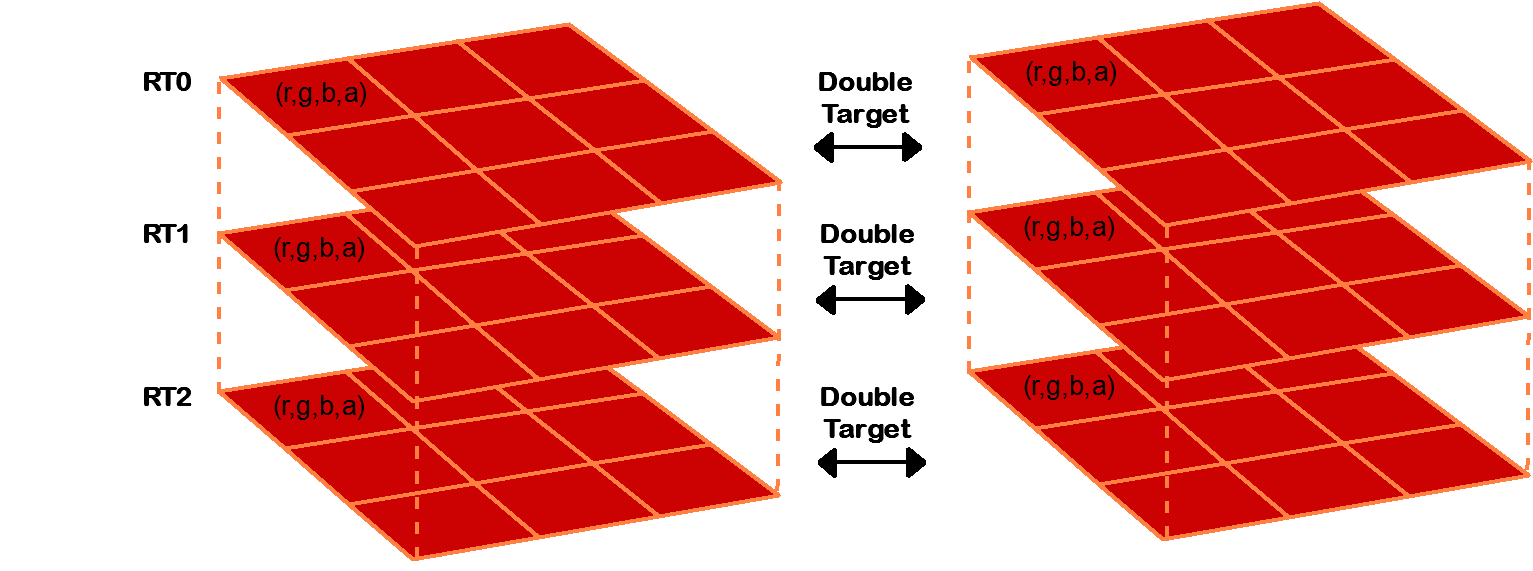
\includegraphics[width=350px]{graphics/DoubleTargets2.png}
	\caption{Duplizierte Rendertargets für Ping-Pong Verfahren.}
	\label{fig:DoubleTarget}
\end{figure}

	\item[Fullscreen-Pass/Offscreen-Pass] \hfill \\
Das Update unserer \textit{Rendertargets} und somit die Manipulation unserer Partikeleigenschaften, findet in einem sogenannten \textit{Fullscreen-Pass} statt, welcher vor dem eigentlichen Zeichen der \textit{Billboards} durchlaufen wird. Hierbei wird ein im \textit{Screenspace} positioniertes, Bildschirmfüllendes Rechteck genutzt, um ein 1-zu-1 Mapping des zu lesenden und des zu schreibenden \textit{Rendertargets} zu erreichen. Da dieser Pass keine Bildschirmausgabe zur folge hat, kann er auch als \textit{Offscreen-Pass} bezeichnet werden.

	\item[Blending] \hfill \\
Um bestimmte Effekte realistischer Darzustellen, bietet das neue Partikelsystem, optional die Möglichkeit, additives Blending (s. Abbildung \ref{fig:addBlending}) zu aktivieren. Dabei werden die Farben übereinanderliegender Partikel aufsummiert, wodurch Bereiche mit vielen übereinanderliegenden Partikeln heller erscheinen (s. Abbildung \ref{fig:particleResults}).

\begin{figure}[h!]
	\centering
	\vspace*{10px}
	
\includegraphics[width=100px]{graphics/additiveBlending.png}
	\caption{Additives Blending.}
	\label{fig:addBlending}
\end{figure}

\end{description}

\newpage
\subsection{Das Ergebnis}

Das Ergebnis unserer Neuimplementierung war mehr als zufriedenstellend. Am Ende hatten wir ein, vom restlichen System getrenntes und sehr flexibles Partikelsystem entwickelt, welches nun komplett auf der GPU lief und uns somit wieder mehr Ressourcen für andere Aufgaben, auf Seiten der CPU zur Verfügung standen. Auch unser, am Anfang noch für utopisch gehaltenes Ziel, eine Anzahl von über 1.000.000 Partikel in Echtzeit darzustellen, konnten wir mit dem neuen System erreichen. Bei über 1.000.000 Partikeln, läuft unsere Anwendung nun immer noch mit über 100 Frames die Sekunde, solche Ergebnisse konnten wir bei der vorherigen CPU-basierten Implementierung, selbst mit minimaler Anzahl an Partikeln nicht erreichen. Abbildung \ref{fig:particleResults} zeigt das Partikelsystem mit einigen unterschiedlichen Konfigurationen.

\begin{figure}[h!]
	\centering
	\vspace*{30px}
	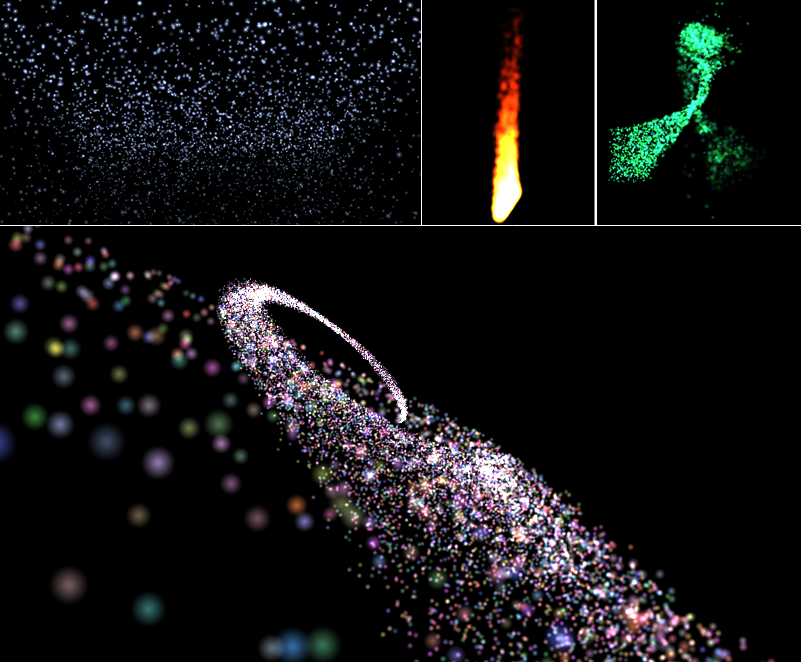
\includegraphics[width=410px]{graphics/ParticleResults.png}
	\caption{Partikelsystem mit unterschiedlichen Konfigurationen.}
	\label{fig:particleResults}
\end{figure}

\end{Spacing}
\newpage
\clearpage
%% End Of Doc